% !TEX TS-program = pdflatexmk
\documentclass{./packages/optica-article}
\graphicspath{{images/}{practica1/images}}
\journal{opticajournal}

\usepackage{csvsimple}
\usepackage{siunitx}
\usepackage{physics}
\usepackage{booktabs}
\usepackage{tikz}

\usepackage{caption}
\usepackage{subcaption}
\usetikzlibrary{positioning}

\newcommand{\sinc}{\textrm{sinc}}
\newcommand\conv{\circledast}

% Set the article type
\articletype{Research Article}
\begin{document}

\title{Caracterización de sistemas de formación de imágenes}

\author{Adriana Mamani Lazarte\authormark{1} Alex G. Recuenco\authormark{1}, and Carlos España Castaño\authormark{1}}

\address{\authormark{1}Universidad Complutense de Madrid, Madrid, CP 28040, España}

\section{Introducción}
En esta práctica vamos a caracterizar un sistema de formación de imágenes mediante la determinación experimental de su función de transferencia de modulación (MTF). Para ello utilizaremos un método directo (el test de barras) y un método indirecto (el test de borde).


\section{Marco práctico}
El sistema cuya MTF mediremos consiste en un objetivo de microscopio con apertura numérica $\textrm{NA} = 0,25$ y un aumento $10\times$ (F10),
y una cámara CCD con un tamaño de píxel de $s=4,65 \unit{\micro\meter}$.
Las imágenes captadas por la cámara se visualizarán en la pantalla del PC.

\subsection{Medida de MTF mediante el test de barras (método directo)}\label{sec:directo}

\begin{figure}[h]
	\centering
	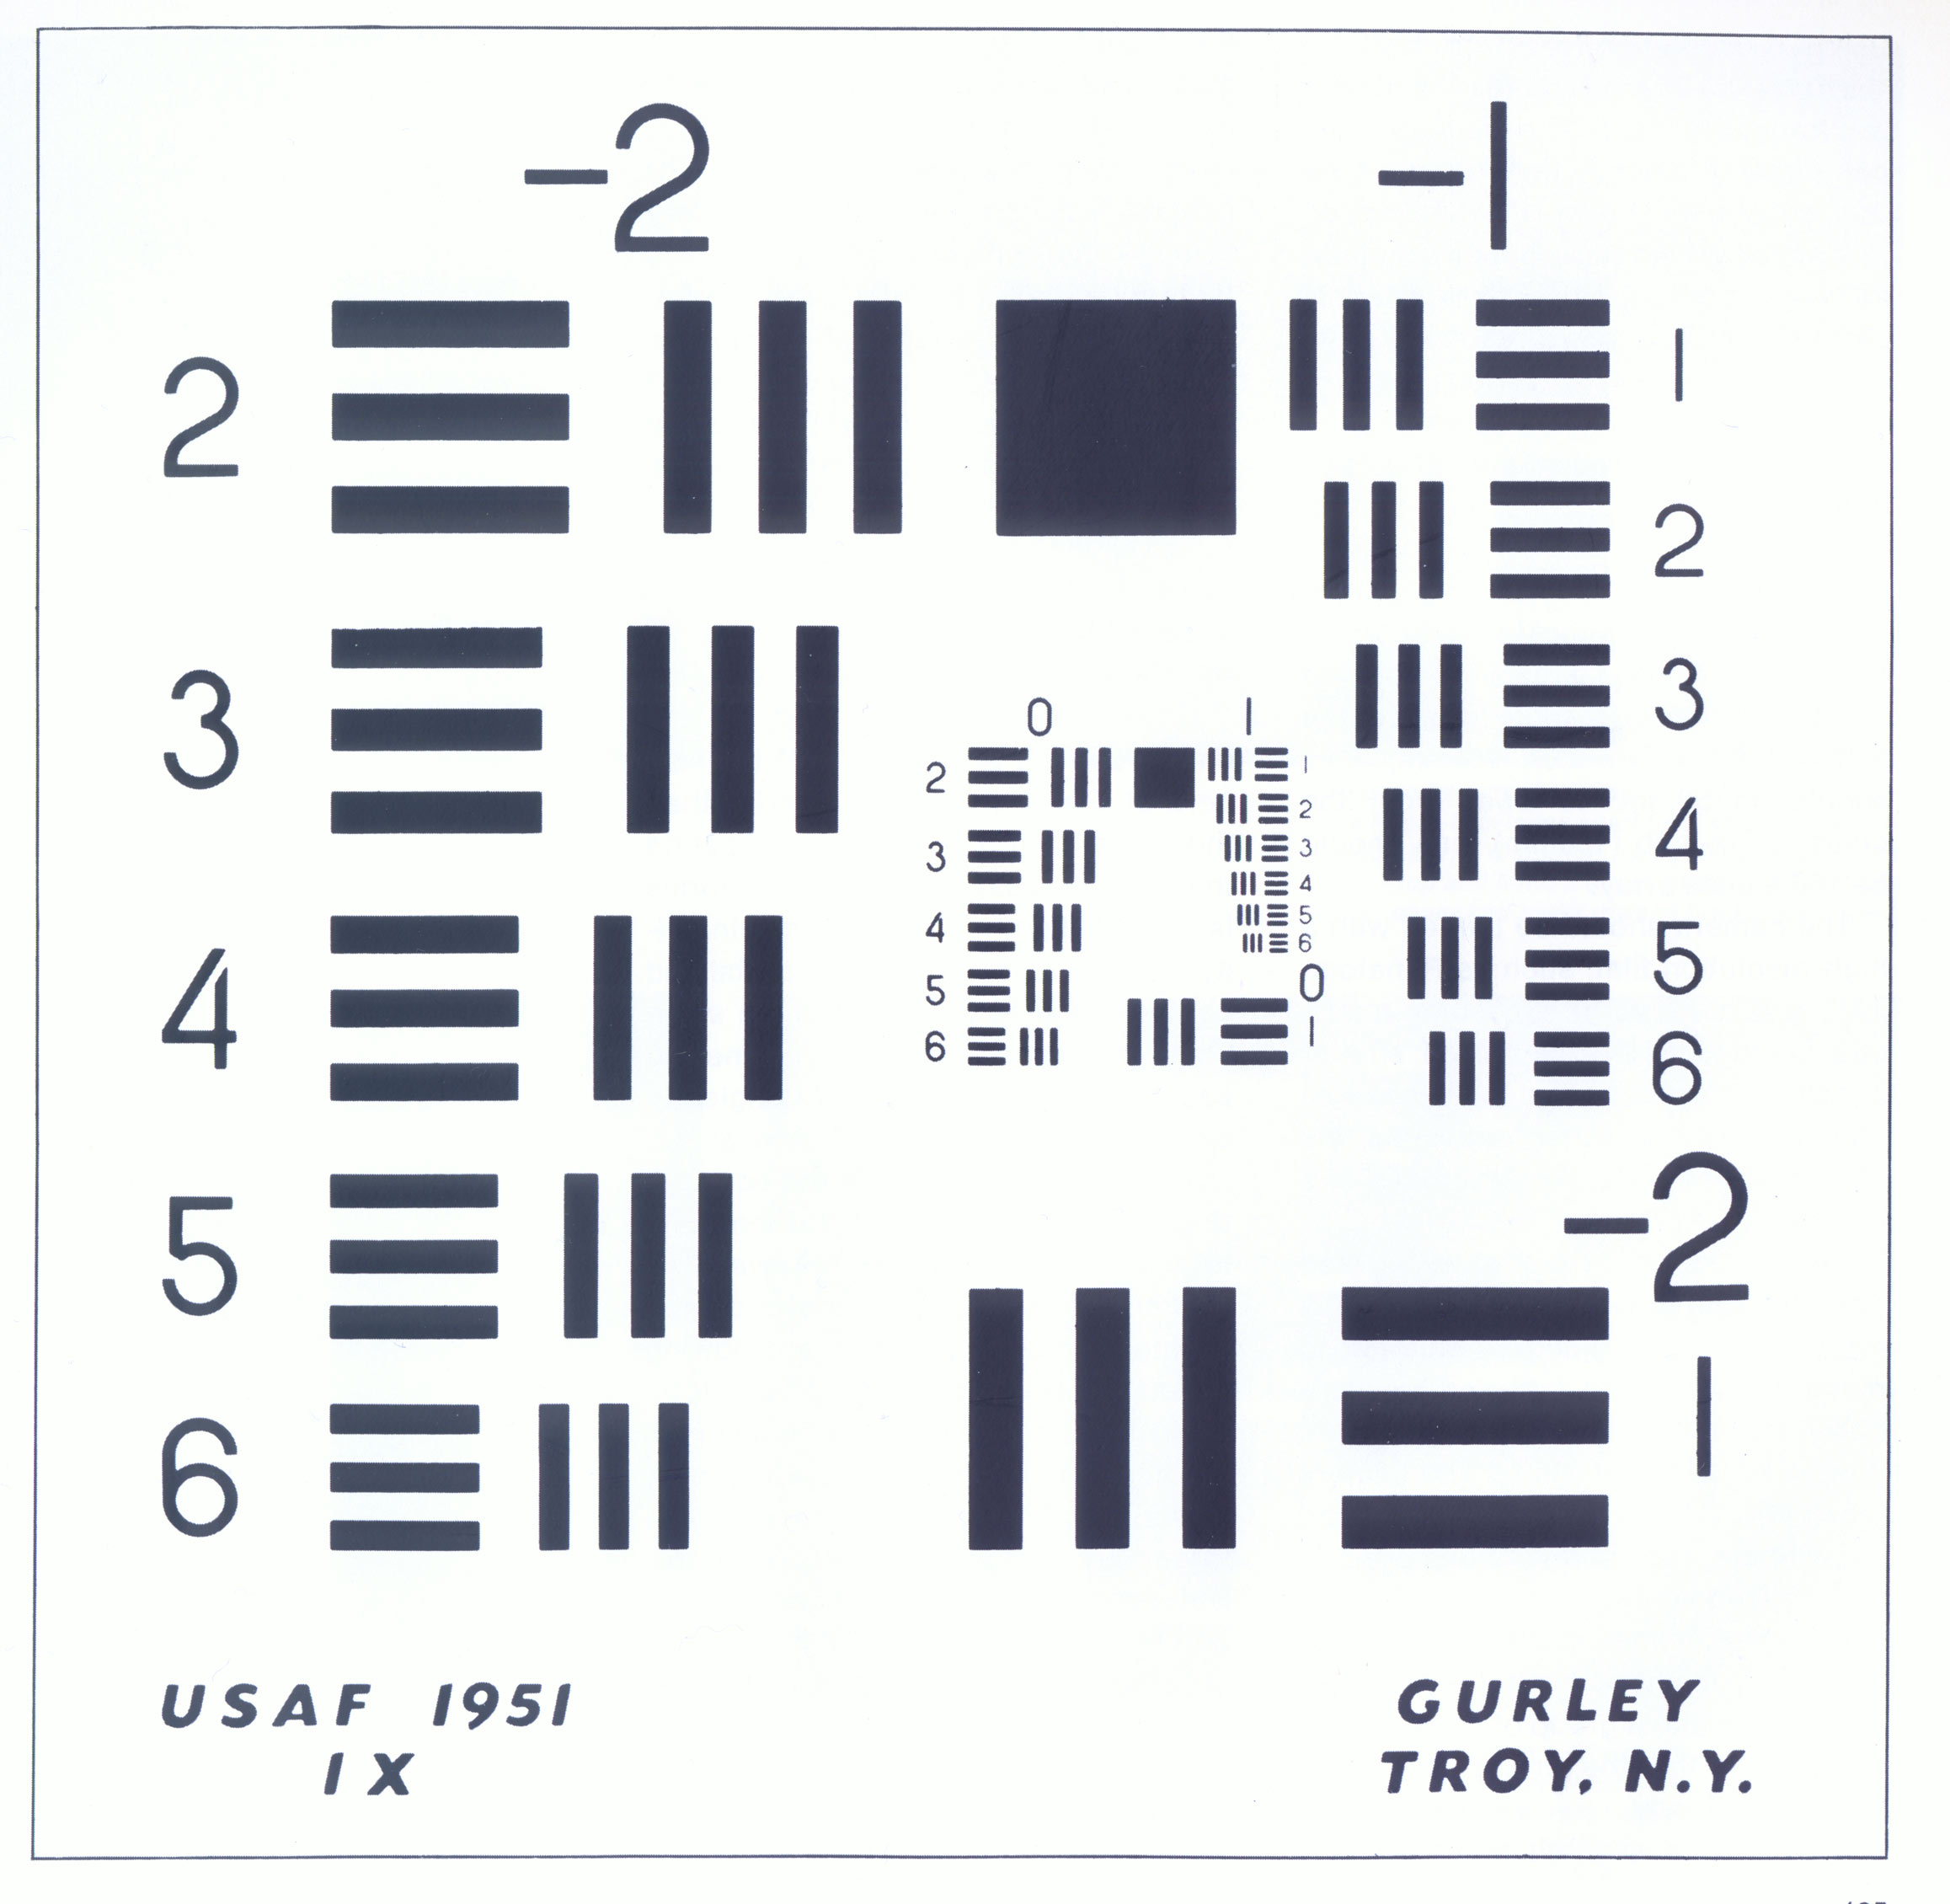
\includegraphics[scale=0.05]{testusaf1951}
	\caption{Test USAF 1951.}\label{fig:usaf1951}
\end{figure}

Utilizando el test USAF 1951 (Fig.~\ref{fig:usaf1951}), y realizamos fotos de cada uno de los distintos elementos de rendijas de la diapositiva, como se indica en la Fig.~\ref{fig:usafpic} presentada a continuación. Se controla la exposición para obtener los colores grises sin sobre-exposición.

\begin{figure}[!h]
	\centering
	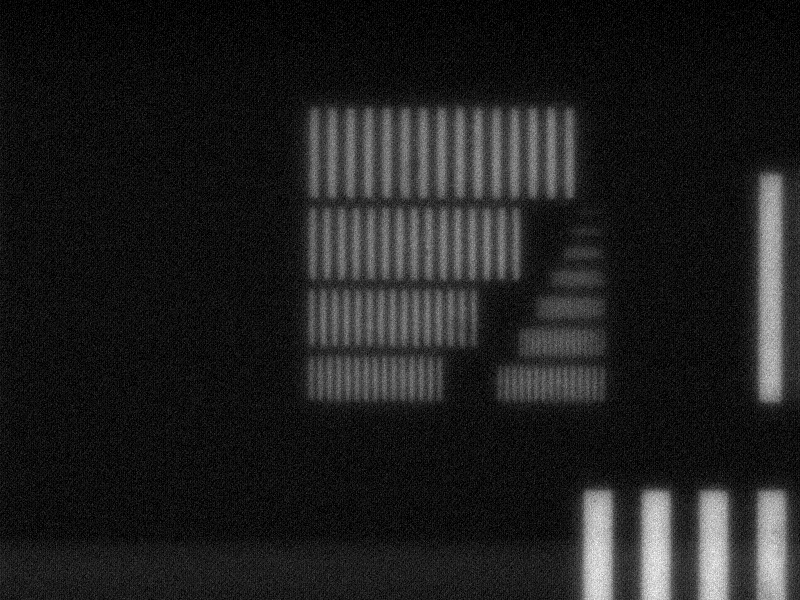
\includegraphics[width=0.5\textwidth]{smallest_lines}
	\caption{Foto tomada durante la práctica de las líneas centrales del test USAF 1951}\label{fig:usafpic}
\end{figure}

Después, se obtiene a través de estas imágenes un perfíl ortogonal a las rendijas de contraste como se indica en Fig.~\ref{fig:example} para cada una de las distintas imágenes. Los resultados se discutirán en la sección~\ref{sec:mtf-directo}.



El contraste se ha obtenido a partir de la expresión:
\nopagebreak
\begin{equation}
	C = \frac{y_{\max} - y_{\min}}{y_{\max} + y_{\min}}.
	\label{eq:contraste}
\end{equation}

La frecuencia se calcula como:
\nopagebreak
\begin{equation}
	\nu = \frac{1825}{T}\ \textrm{ciclos/mm},\quad\textrm{TODO: QUE es 1825??}\label{eq:frecuencia}
\end{equation}

Donde el periodo, $T$, se calcula como se explica en Fig.~\ref{fig:perfil:example}.

\subsection{Medida de la MTF mediante el test de borde (método indirecto)}\label{sec:description:indirecto}

Se obtiene la imagen de una única barra que abarque el campo completo de visión, dividiendo la imagen ortogonalmente como se puede ver en la Fig.~\ref{fig:perfil:img}

\begin{figure}[hptb]
	\centering
	\begin{subfigure}[t]{0.31\textwidth}
		\centering
		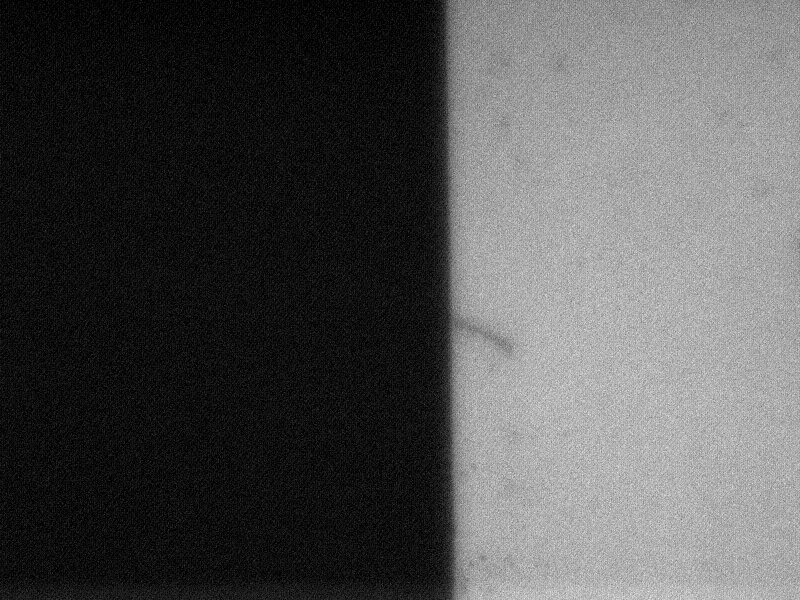
\includegraphics[width=\textwidth]{edge_large_line}
		\caption{Imagen de una franja amplia}\label{fig:perfil:img}
	\end{subfigure}
	\hfill
	\begin{subfigure}[t]{0.31\textwidth}
		\centering
		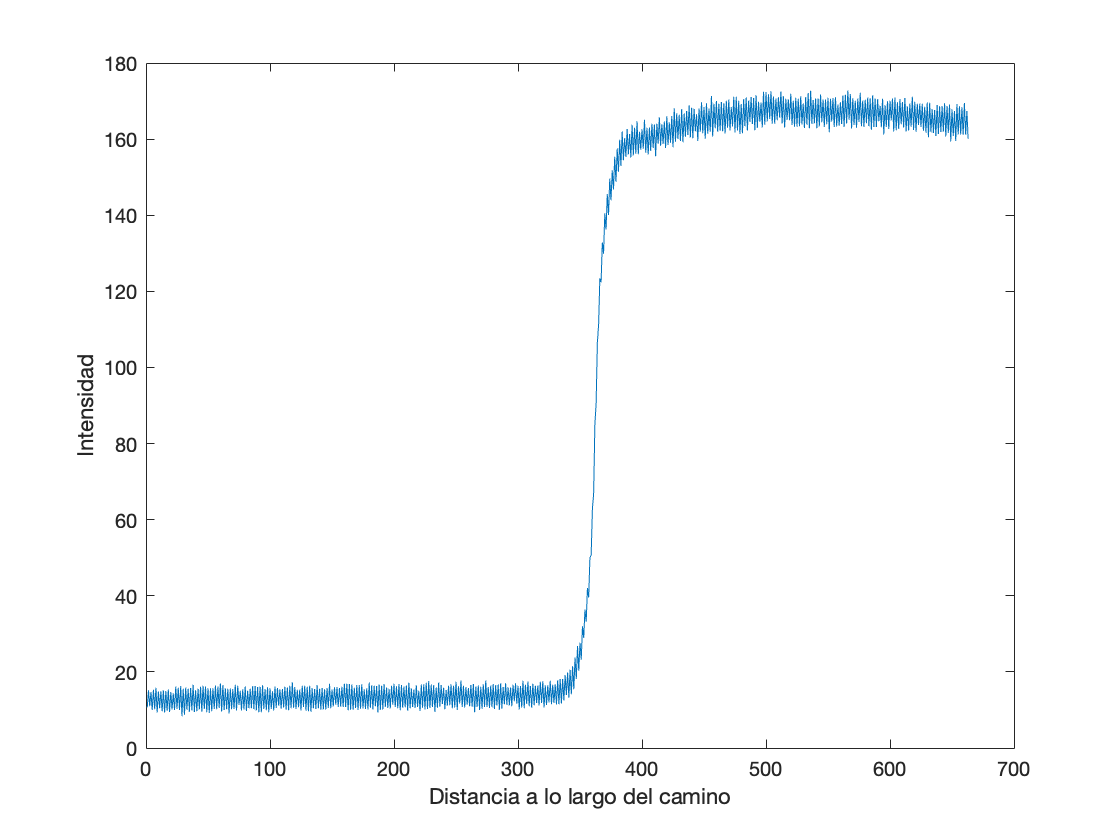
\includegraphics[width=\textwidth]{edge_perfil}
		\caption{Perfil de intensidad de píxeles en una línea horizontal}\label{fig:perfil:graph}
	\end{subfigure}
	\hfill
	\begin{subfigure}[t]{0.31\textwidth}
		\centering
		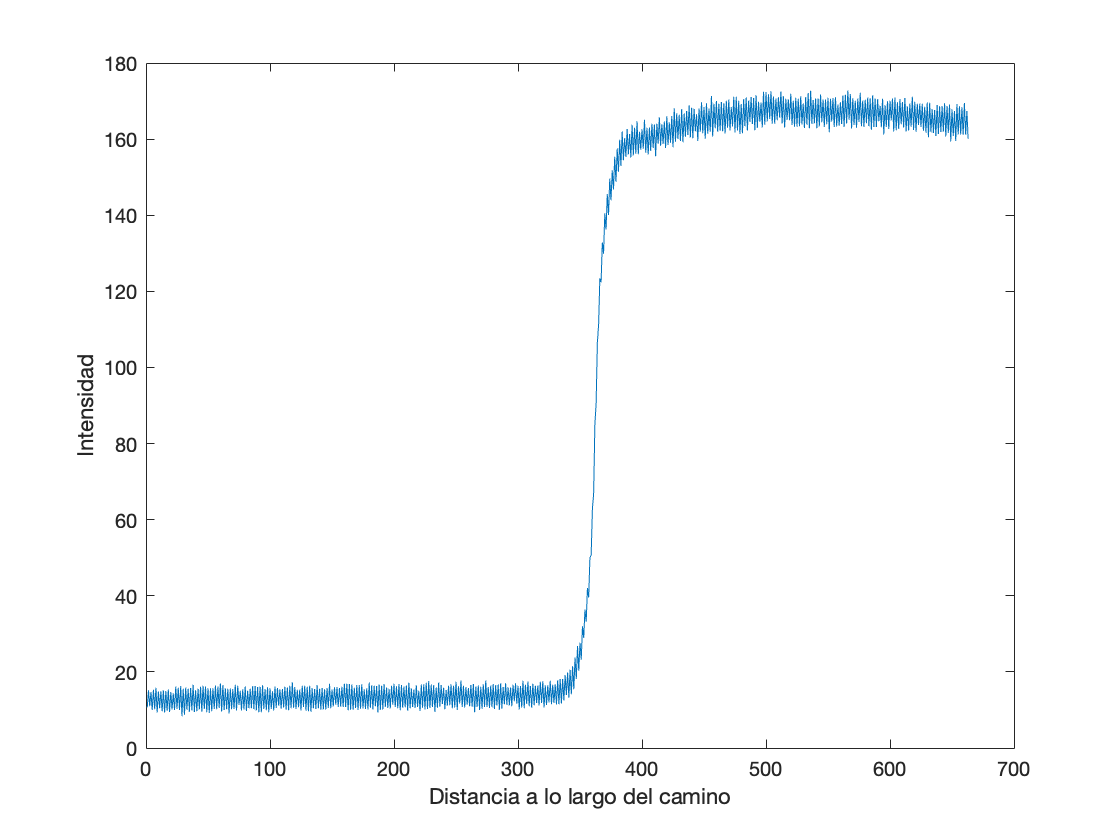
\includegraphics[width=\textwidth]{edge_perfil}
		\caption{TODO: Imagen de la derivada del perfil}\label{fig:perfil:lsf}
	\end{subfigure}

	\caption{Perfil de intensidad de una franja grande utilizada para el método indirecto para obtener el MTF, como se describe en la sección~\ref{sec:description:indirecto}}\label{fig:perfil}
\end{figure}

\section{Resultados experimentales}\label{sec:resultados}

\subsection{Medida de la MTF mediante el test de barras (método directo)}\label{sec:resultados:directo}
Se realizó el procedimiento explicado en Fig.~\ref{fig:perfil:example} por cada imagen que se obtuvo del test de USAF (Fig.~\ref{fig:usaf1951}) durante la practica (Fig.~\ref{fig:images:example}).

\begin{figure}[!h]
	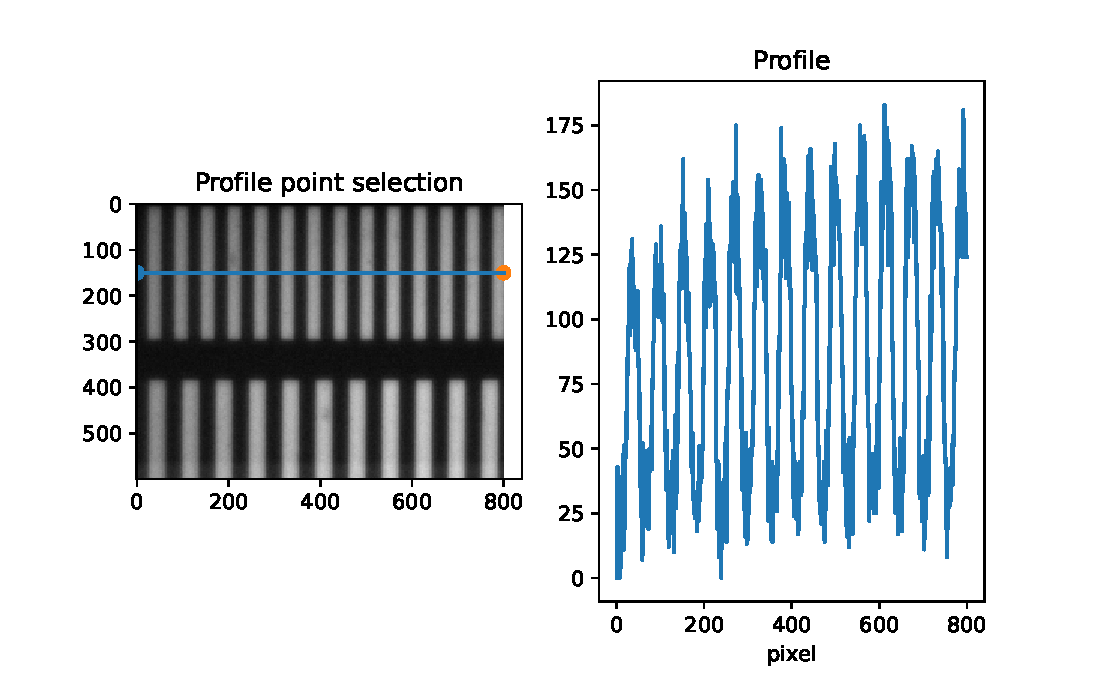
\includegraphics[width=\textwidth]{profile-lines.pdf}
	\caption{Procedimiento para sacar el perfil de un segmento de líneas. Se obtiene dos posiciones tan distantes como se pueda de dos mínimos de las barras. Se mide la distancia en píxeles entre ellas ($x_{\max} - x_{\min} $), se cuenta el número de periodos entre ellas, que nos permite calcular $T = \flatfrac{x_{\max} - x_{\min} }{N_{\textrm{periodos}}}$. A continuación,  se toma los máximos y mínimos de altura $y_{\max}$, $y_{\min}$, que nos permite calcular el contraste usando la formula~\ref{eq:contraste} }\label{fig:perfil:example}
\end{figure}

A continuación se muestran algunas de las imágenes de las tomadas en la PC en esta sección:

\begin{figure}[!h]
	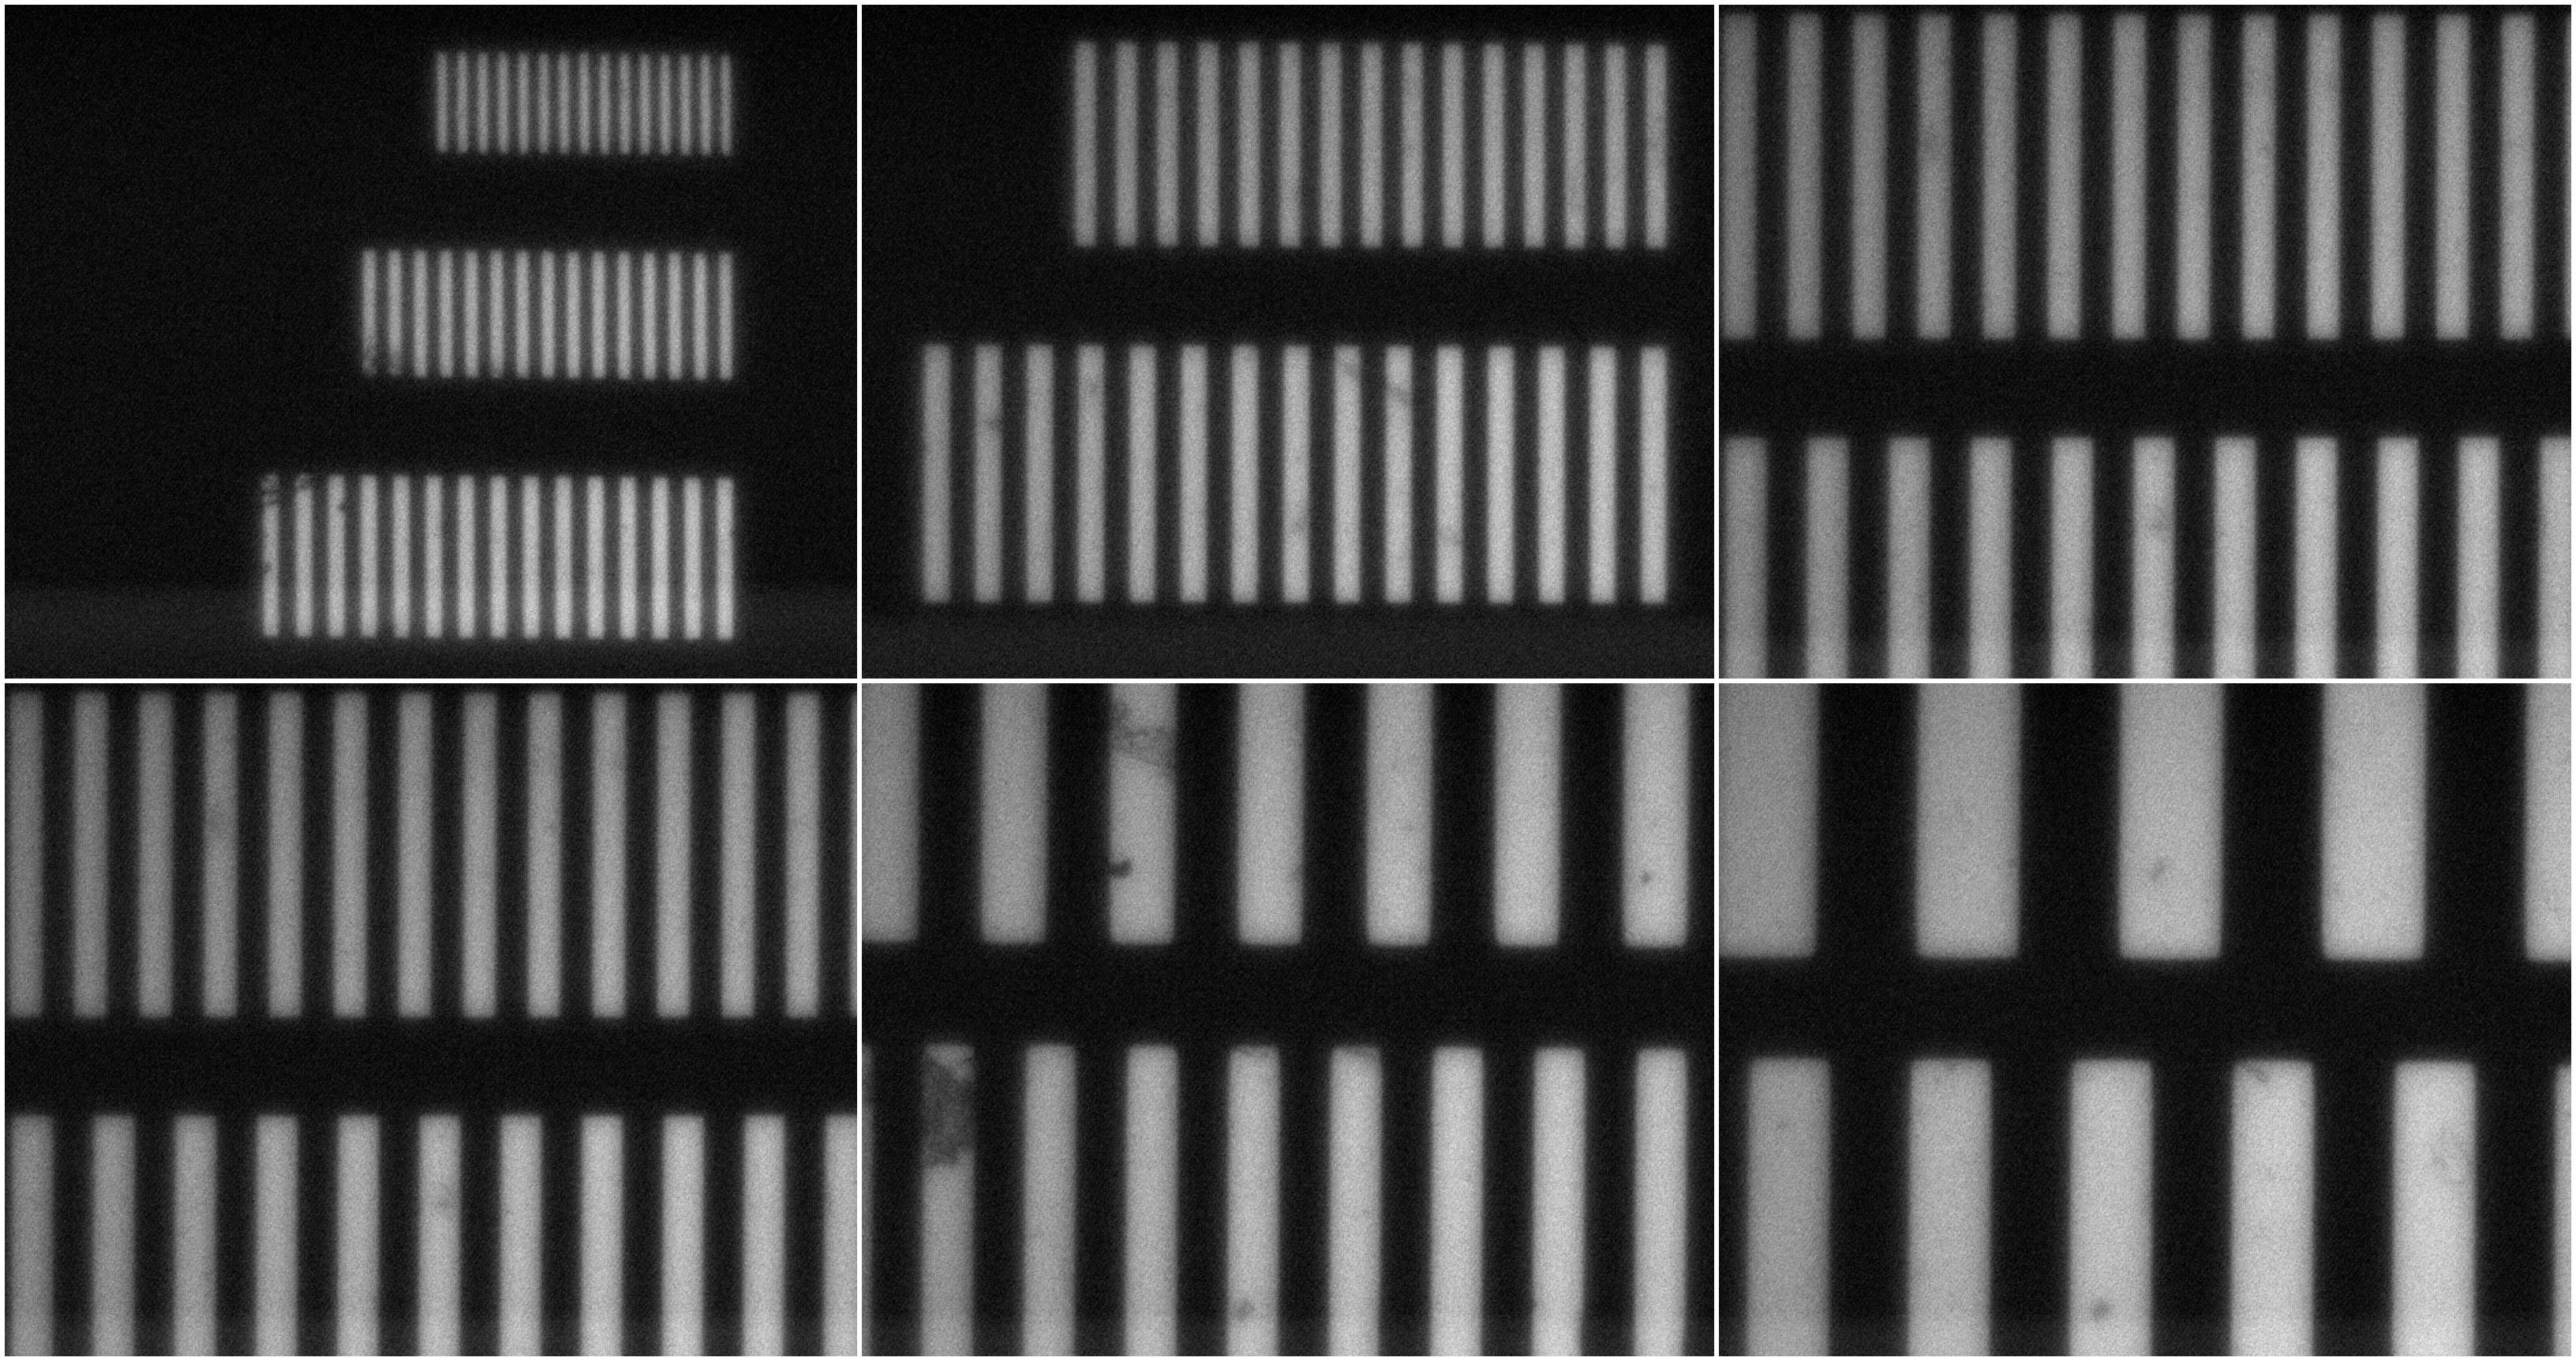
\includegraphics[width=0.9\textwidth]{/imaglineas.jpg}
	\caption{Imágenes tomadas del test de USAF Fig.~\ref{fig:usaf1951} para la medida del MTF directo}\label{fig:images:example}
\end{figure}


En la tabla~\ref{table:perfilintensidad} se recogen medidas tomadas del perfil de intensidad para distintos conjuntos de barras, posterior a obtener los datos del perfil de las imágenes.

\begin{table}[p]
	\centering
	\csvautotabular[
		table head=\toprule%
		Barras & $y_{\min} (px)$ & $y_{\max} (px)$ & Contraste & $x_{\min} (px)$ & $x_{\max} (px)$ & N Periodos & periodo (px) &  $\flatfrac{\textrm{ciclos}}{\textrm{mm}}$%
		\\\midrule%
	]{practica1/MTF/Profiles.csv}
	\caption{Datos del perfil de intensidad. $y$: intensidad. $x$: distancia en píxeles. El contraste se ha obtenido a partir de la ecuación~\ref{eq:contraste}.
		la frecuencia se ha obtenido a través de la equacion~\ref{eq:frecuencia}}%
	\label{table:perfilintensidad}
\end{table}





\subsection{Medida de la MTF mediante el test de borde (método indirecto)}\label{sec:resultados:indirecto}

Debido a que la función $\delta(x)$ es la derivada de la step function, $s(x)$, como distribución, podemos usar este hecho para calcular la LTF, encontrando primero la respuesta a un borde, y realizando una estimación de la derivada, podemos obtener la LTF más fácilmente

\section{Cuestiones}

\subsection{Sea $H_{c}(u)$ la función de transferencia de un sistema para luz coherente. Escribir la relación entre $H_{c}(u)$ y la función de transferencia del mismo sistema para luz incoherente, $H_{i}(u)$.}

Cuando la luz incidente es coherente, la imagen resultante se obtiene añadiendo linealmente la amplitud compleja. Sin embargo, cuando la iluminación es idealmente incoherente, la iluminación es linear en la intensidad de la onda incidente. Por ello, en el caso ideal donde la correlación de fase es cero para distintas posiciones, se obtiene que~\cite[p.~132--134]{goodman1996introduction}.

\begin{equation}
	I_{i}(u,v) = \kappa \iint_{-\infty}^{\infty}\abs{h(u - \xi, v- \eta)}^{2} I_{g}(\xi, \eta) \dd \xi \dd \eta.
\end{equation}

Por lo tanto, la función $H_{i}(u)$ se puede obtener con el esquema descrito en Fig.~\ref{fig:transformacion}. Básicamente, haciendo la transformación inversa para obtener $h_{c}$, luego multiplicando está con su conjugada, obteniendo $h_{i}$, donde $i$ denota intensidad. Y al realizar la transformada inversa obtenemos el resultado.

\begin{align*}
	H_{i}(u)
	 & = TF\{h_i\}
	= TF\left\{ h_{c} \cdot h^{*}_{c}\right\}
	= TF\left\{ h_{c} \cdot h^{*}_{c}\right\}
	= TF\left\{ TF^{-1}\{H_{c}\} \cdot {TF^{-1}\{H_{c}\}}^{*}\right\}
	\\
	 & = H_{c} \conv H^{*}_{c}. %
	% Numerar sólo la última equación.
	\addtocounter{equation}{1}\tag{\theequation} \label{eq:incoherent-conv}
\end{align*}

\begin{figure}[htpb]
	\begin{center}
		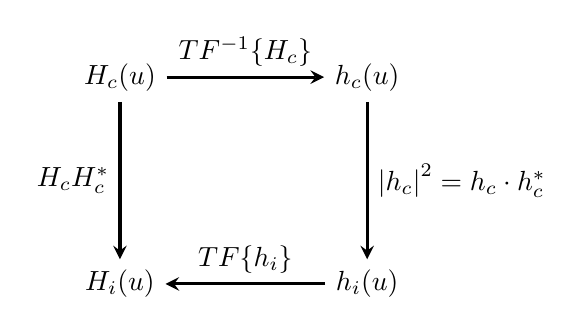
\begin{tikzpicture}[line width=0.4mm, >=stealth]

			\def \n {5}
			\def \radius {3cm}
			\def \margin {8} % margin in angles, depends on the radius

			\node (H) at (0,0) {$H_{c}(u)$};
			\node[right=2cm of H] (h) {$h_{c}(u)$};
			\node[below=2cm of h] (hi) {$h_{i}(u)$};
			\node[below=2cm of H] (Hi) {$H_{i}(u)$};
			\draw[->] (H) -- (h) node[pos=0.5, anchor=south] {$TF^{-1}\{H_{c}\}$};
			\draw[->] (h) -- (hi) node[pos=0.5, anchor=west] {$\abs{h_{c}}^{2} = h_{c} \cdot h^{*}_{c}$};
			\draw[->] (hi) -- (Hi) node[pos=0.5, anchor=south] {$TF\{h_{i}\}$};
			\draw[->] (H) -- (Hi) node[pos=0.5, anchor=east] {$H_{c} \conv H^{*}_{c}$};
		\end{tikzpicture}
	\end{center}
	\caption{Diagrama TODO, describirlo mejor}\label{fig:transformacion}
\end{figure}

\subsection[]{Para un sistema parecido al usado en la práctica:
	\begin{enumerate}
		\item Estimar la frecuencia de corte de la cámara CCD, $u_{c}^{(CCD)}$, en líneas por milímetro.
		\item Estimar la frecuencia de corte $u_{c}^{(Obj)}$ del objetivo $10\times$ para luz incoherente (la longitud de onda media $\lambda=500\,\unit{\nano\metre}$).
		\item Tomando estos valores y suponiendo que la PSF del objetivo y de la cámara se aproximan por la función $|\sinc(ax)|^2$, dibujar la MTF de cada uno de los elementos y del sistema compuesto.
	\end{enumerate}
}




\subsection{Aplicar usando el plugin Deconvolutionlab2 y Image J dos métodos de convolución: Regularized Inverse Filter y Richardson-Lucy a una imagen test obtenida por un sistema con una PSF conocida y diferentes tipos de ruido: Guass y Poisson.}

Comenzamos con una imagen como se describe en Fig.~\ref{fig:image:ref-psf}

Convolution Noiseless (convolución sin ruido);

b) Simulation with noise-Gauss (convolución con ruido Gaussiano:
Mean=0
Stdev: 0.1 y 0.01 );

c) Simulation with noise-Poisson (Convolución con ruido Poisson 0.01, 10 y 0.0001, las dos ultimas no
hace falta deconvoluciones después ) y guardar las imágenes correspondientes como  `refconv',  `refNG'\ldots y  `refNP' como \verb|.TIF| o \verb|.BMP|.
Nivel de ruido:
Aplicar los algoritmos de deconvolución a las imágenes obtenidas en el apartado anterior (arrastrar a la ventana `Image'):
a) Regularized Inverse filter:
RIF: =0.01, =1.
b) Richardson-Lucy (RL) algorithm con 10 y 50 iteraciones. Probar 100 iteraciones para una caso y comparar con 50 iteraciones



\begin{figure}[hbp]
	\centering
	\begin{subfigure}[t]{0.45\textwidth}\centering
		\centering
		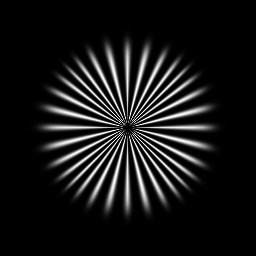
\includegraphics[width=\textwidth]{Simulation deconvolution/ref.jpg}
		\caption{Imagen referencia test original}\label{fig:ref}
	\end{subfigure}
	\hfill
	\begin{subfigure}[t]{0.45\textwidth}\centering
		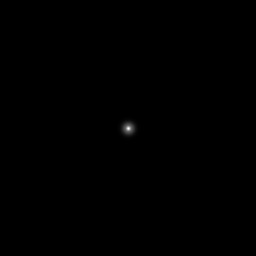
\includegraphics[width=\textwidth]{Simulation deconvolution/psf.jpg}
		\caption{Imagen PSF}\label{fig:psf}
	\end{subfigure}

	\caption{Imagen usada para la simulación con Deconvolutionlab2 y Image J, y el PSF del systema de captura simulado}\label{fig:image:ref-psf}
\end{figure}

\begin{figure}[hbp]
	% Esto no se hace asi con hfill y \, ... pero no me acuerdo como
	\begin{center}
		\,\hfill
		\begin{subfigure}[t]{0.25\textwidth}\centering
			\centering
			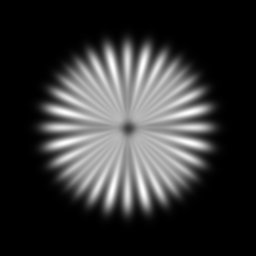
\includegraphics[width=\textwidth]{Simulation deconvolution/ref_conv}
			\caption{Convolution}\label{fig:sim:conv}
		\end{subfigure}
		\,\hfill
		\begin{subfigure}[t]{0.25\textwidth}\centering
			\centering
			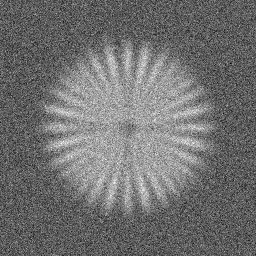
\includegraphics[width=\textwidth]{Simulation deconvolution/ref_ng_0.1}
			\caption{Convolution ng 0.1}\label{fig:sim:ng0.1}
		\end{subfigure}
		\hfill
		\begin{subfigure}[t]{0.25\textwidth}\centering
			\centering
			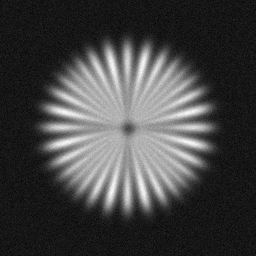
\includegraphics[width=\textwidth]{Simulation deconvolution/ref_ng_0.01}
			\caption{Convolution ng 0.01}\label{fig:sim:ng0.01}
		\end{subfigure}
		\hfill\,
		\\
		\hfill\,
		\begin{subfigure}[t]{0.25\textwidth}\centering
			\centering
			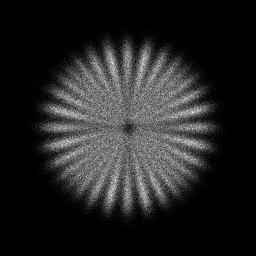
\includegraphics[width=\textwidth]{Simulation deconvolution/ref_np_0.01}
			\caption{NP 0.01}\label{fig:sim:np0.01}
		\end{subfigure}
		\hfill
		\begin{subfigure}[t]{0.25\textwidth}\centering
			\centering
			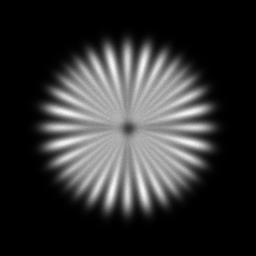
\includegraphics[width=\textwidth]{Simulation deconvolution/ref_np_0.0001}
			\caption{NP 0.0001}
		\end{subfigure}
		\hfill
		\begin{subfigure}[t]{0.25\textwidth}\centering
			\centering
			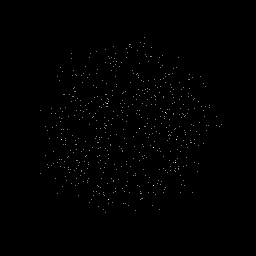
\includegraphics[width=\textwidth]{Simulation deconvolution/ref_np_10}
			\caption{NP 10}
		\end{subfigure}
		\hfill\,
		\caption{Simulación usando~\ref{fig:image:ref-psf} con distintos algoritmos para simular el ruido}\label{fig:convolutions}
	\end{center}
\end{figure}
\begin{figure}
	\centering
	\begin{tabular}[t]{l c c c c}
		Original Image                                                                  & RIF 0.01 & RIF 1 & RL 10 & RL 50 \\
		Fig.~\ref{fig:sim:conv}                                                         &
		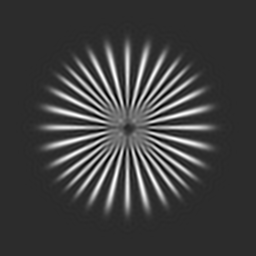
\includegraphics[scale=0.25]{Simulation deconvolution/ref_conv/RIF_0.01.png}    &
		
\includegraphics[scale=0.25]{Simulation deconvolution/ref_conv/RIF_1.png}       &
		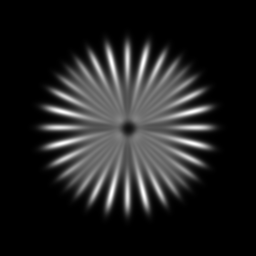
\includegraphics[scale=0.25]{Simulation deconvolution/ref_conv/RL_10.png}       &
		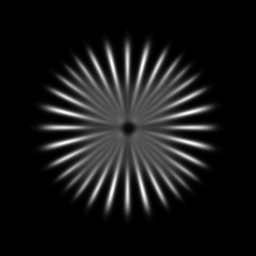
\includegraphics[scale=0.25]{Simulation deconvolution/ref_conv/RL_50.png}
		\\
		Fig.~\ref{fig:sim:ng0.1}                                                        &
		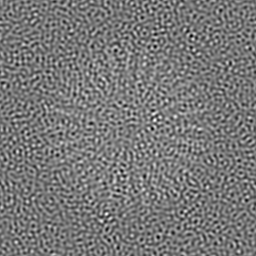
\includegraphics[scale=0.25]{Simulation deconvolution/ref_ng_0.1/RIF_0.01.png}  &
		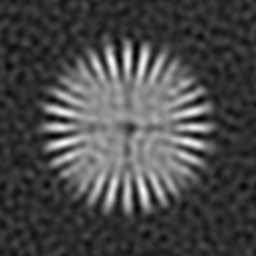
\includegraphics[scale=0.25]{Simulation deconvolution/ref_ng_0.1/RIF_1.png}     &
		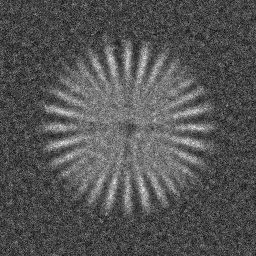
\includegraphics[scale=0.25]{Simulation deconvolution/ref_ng_0.1/RL_10.png}     &
		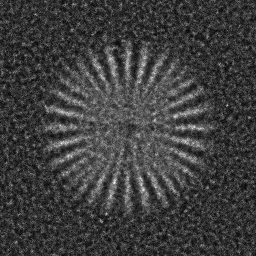
\includegraphics[scale=0.25]{Simulation deconvolution/ref_ng_0.1/RL_50.png}
		\\
		Fig.~\ref{fig:sim:ng0.01}                                                       &
		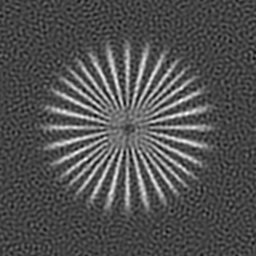
\includegraphics[scale=0.25]{Simulation deconvolution/ref_ng_0.01/RIF_0.01.png} &
		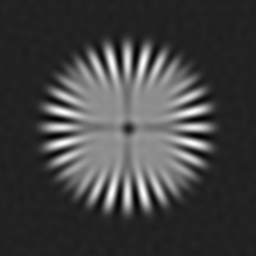
\includegraphics[scale=0.25]{Simulation deconvolution/ref_ng_0.01/RIF_1.png}    &
		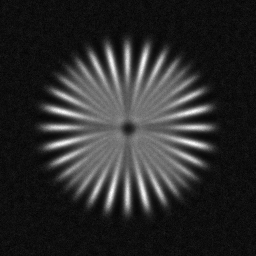
\includegraphics[scale=0.25]{Simulation deconvolution/ref_ng_0.01/RL_10.png}    &
		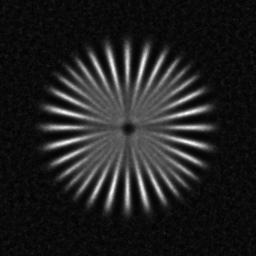
\includegraphics[scale=0.25]{Simulation deconvolution/ref_ng_0.01/RL_50.png}
		\\
		Fig.~\ref{fig:sim:np0.01}                                                       &
		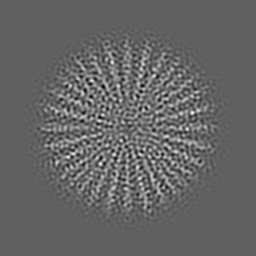
\includegraphics[scale=0.25]{Simulation deconvolution/ref_np_0.01/RIF_0.01.png} &
		
\includegraphics[scale=0.25]{Simulation deconvolution/ref_np_0.01/RIF_1.png}    &
		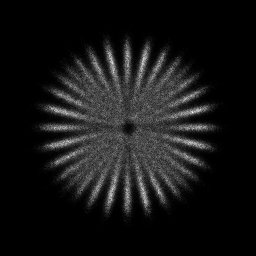
\includegraphics[scale=0.25]{Simulation deconvolution/ref_np_0.01/RL_10.png}    &
		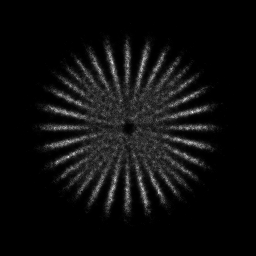
\includegraphics[scale=0.25]{Simulation deconvolution/ref_np_0.01/RL_50.png}
		\\
	\end{tabular}
	\caption{Matriz de de-convoluciones para cada uno de las de-convoluciones indicadas en las imagenes \ref{fig:convolutions}.
		TODO: Indicar mas lo que sea
	}
\end{figure}


%%%%%%%%%% If using BibTeX:
\bibliography{bibliography}

\end{document}
